\documentclass{beamer}
\usepackage[utf8]{inputenc}
\usepackage{graphicx}

\newtheorem{definicion}{Definición}
\newtheorem{ejemplo}{Ejemplo}

%%%%%%%%%%%%%%%%%%%%%%%%%%%%%%%%%%%%%%%%%%%%%%%%%%%%%%%%%%%%%%%%%%%%%%%%%%%%%%%
\title[Presentación con Beamer]{Polinomio Interpolador de Newton}
\subtitle[Presentación con Beamer]{$f(x)=sin(x)$}
\author[Técnicas Experimentales]{Francisco Javier Reyes Sánchez \\Zoilo González García}
\date[25-03-2014]{25 de abril de 2014}
%%%%%%%%%%%%%%%%%%%%%%%%%%%%%%%%%%%%%%%%%%%%%%%%%%%%%%%%%%%%%%%%%%%%%%%%%%%%%%%

%\usetheme{Madrid}
%\usetheme{Antibes}
%\usetheme{tree}
\usetheme{classic}

%%%%%%%%%%%%%%%%%%%%%%%%%%%%%%%%%%%%%%%%%%%%%%%%%%%%%%%%%%%%%%%%%%%%%%%%%%%%%%%
\begin{document}
  
%++++++++++++++++++++++++++++++++++++++++++++++++++++++++++++++++++++++++++++++  
\begin{frame}

  
\includegraphics[width=0.15\textwidth]{img/ullesc}
  \hspace*{7.0cm}
  
\includegraphics[width=0.16\textwidth]{img/fmatesc}
  \titlepage

  \begin{small}
    \begin{center}
     Facultad de Matemáticas \\
     Universidad de La Laguna
    \end{center}
  \end{small}

\end{frame}
%++++++++++++++++++++++++++++++++++++++++++++++++++++++++++++++++++++++++++++++  

%++++++++++++++++++++++++++++++++++++++++++++++++++++++++++++++++++++++++++++++  
\begin{frame}
  \frametitle{Índice}  
  \tableofcontents[pausesections]
\end{frame}
%++++++++++++++++++++++++++++++++++++++++++++++++++++++++++++++++++++++++++++++  


\section{Interpolador Polinómico}


%++++++++++++++++++++++++++++++++++++++++++++++++++++++++++++++++++++++++++++++  
\begin{frame}

\frametitle{Interpolador Polinómico}

 \begin{itemize}
 \item
    En análisis numérico, la interpolación polinomica es una técnica de interpolación de un conjunto de datos o de una función por un polinomio. 
 \item
    El objetivo de esta técnica es el de hallar un polinomio que permita hallar aproximaciones de valores desconocidos para la función.
  \end{itemize}

\end{frame}
%++++++++++++++++++++++++++++++++++++++++++++++++++++++++++++++++++++++++++++++  

\section{Cálculo del Polinomio Interpolador de Newton}

%++++++++++++++++++++++++++++++++++++++++++++++++++++++++++++++++++++++++++++++  
\begin{frame}

\frametitle{Cálculo del Polinomio Interpolador de Newton}
\textbf{Definición:} Sea $f_{n}$  una variable discreta de n  elementos y sea $x_{n}$ otra variable discreta de n elementos los cuales corresponden a la imagen y la abcisa de los datos que se quieren interpolar:
  \[f(x_{k})=f_{k}, \hspace{0.5 cm} k=1,...,n\]
El polinomio de grado n-1  resultante de aplicar este método, tendrá la forma:
\[\sum_{i=0}^{n-1} {a_j}(\prod_{j=1}^{j-1}{(x-x_{i})})\]
\end{frame}
%++++++++++++++++++++++++++++++++++++++++++++++++++++++++++++++++++++++++++++++
\begin{frame}
Los coeficientes $a_{j}$ son las llamadas diferencias divididas.
\[ a_{j}=f[x_{0},x_{1},...,x_{j-1},x_{j},]\]
\end{frame}
%++++++++++++++++++++++++++++++++++++++++++++++++++++++++++++++++++++++++++++++
\section{Procedimiento experimental}

\subsection{Descripción de los experimentos}
%++++++++++++++++++++++++++++++++++++++++++++++++++++++++++++++++++++++++++++++  
\begin{frame}
\frametitle{Descripción de los experimentos}
\begin{itemize}
  \item <1-> Seno
  \item <2-> Polinomio interpolador
  \item <3-> Diferencias divididas
  \item <4-> Comprobación  
\end{itemize}
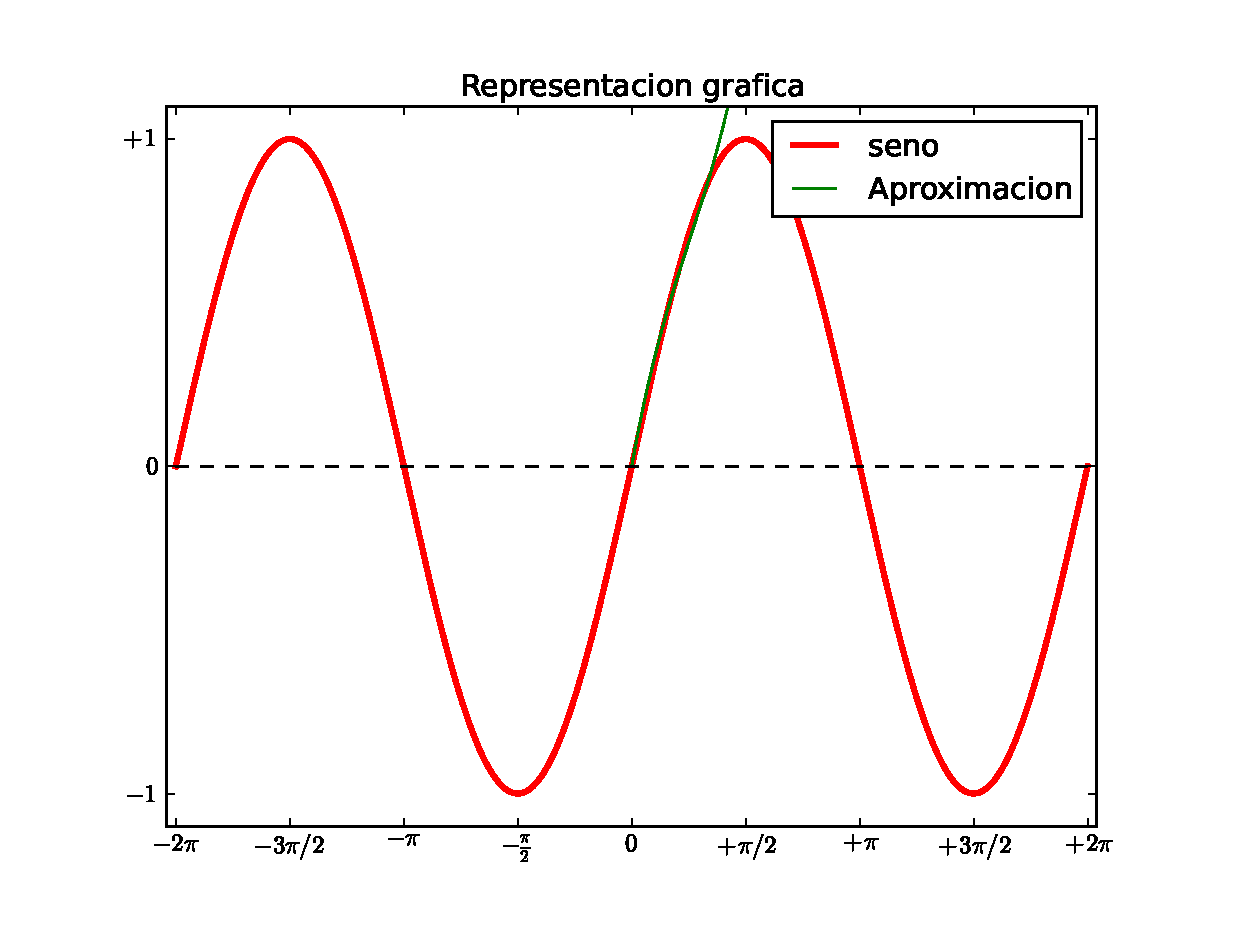
\includegraphics[scale=0.35]{img/representacionseno.eps}
\end{frame}
%++++++++++++++++++++++++++++++++++++++++++++++++++++++++++++++++++++++++++++++  

\subsection{Material}

%++++++++++++++++++++++++++++++++++++++++++++++++++++++++++++++++++++++++++++++  
\begin{frame}
\frametitle{Descripción del material}
\includegraphics[scale=0.25]{img/portatil.eps}

\includegraphics[scale=0.15]{img/bardinux.eps}

\end{frame}
%++++++++++++++++++++++++++++++++++++++++++++++++++++++++++++++++++++++++++++++  

\subsection{Resultados}
%++++++++++++++++++++++++++++++++++++++++++++++++++++++++++++++++++++++++++++++  
\begin{frame}
\frametitle{Análisis de los resultados obtenidos}
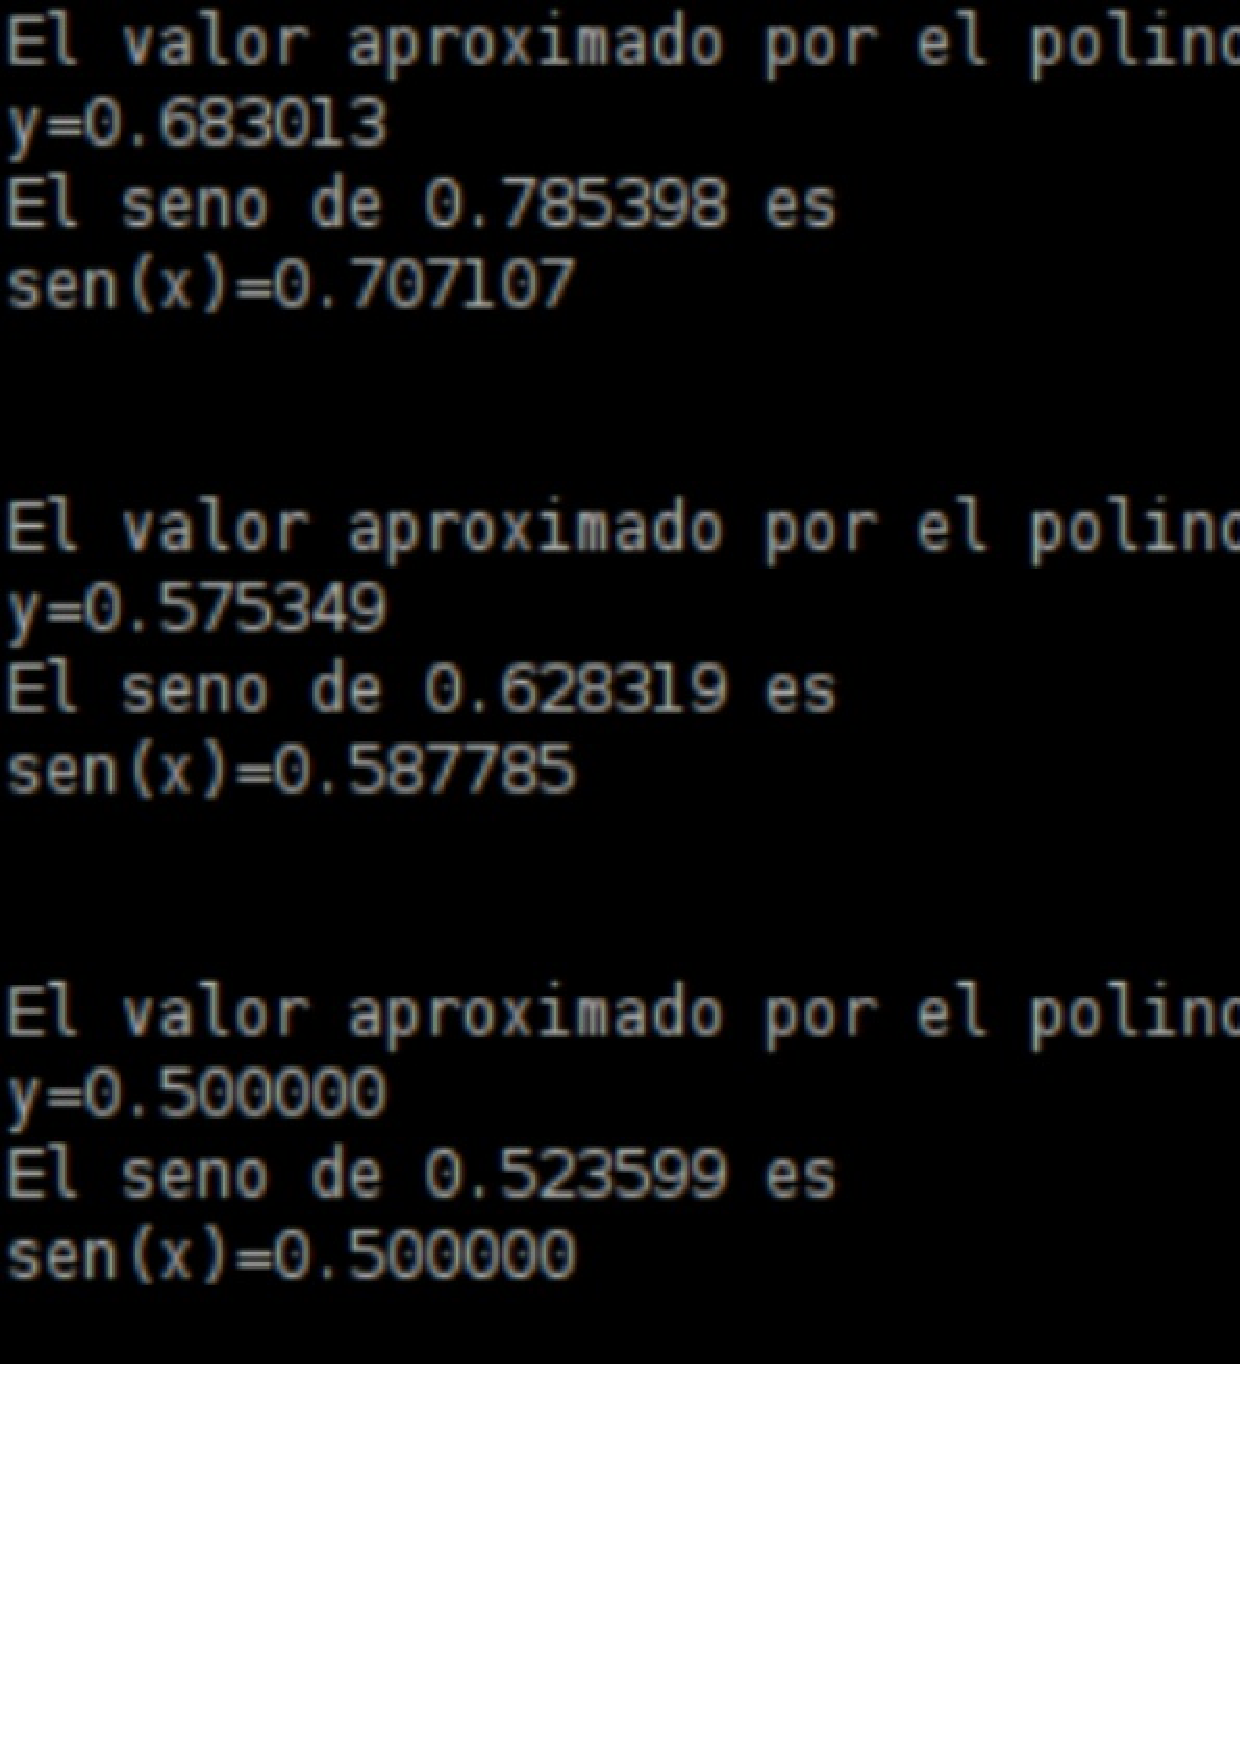
\includegraphics[width=0.5\textwidth]{img/comprobacion}
\end{frame}
%++++++++++++++++++++++++++++++++++++++++++++++++++++++++++++++++++++++++++++++  
%+++++++++++++++++++++++++++++++++++++++++++++++++++++++++++++++++++++++++++++
\section{Algoritmos}
%++++++++++++++++++++++++++++++++++++++++++++++++++++++++++++++++++++++++++++++  
\begin{frame}
  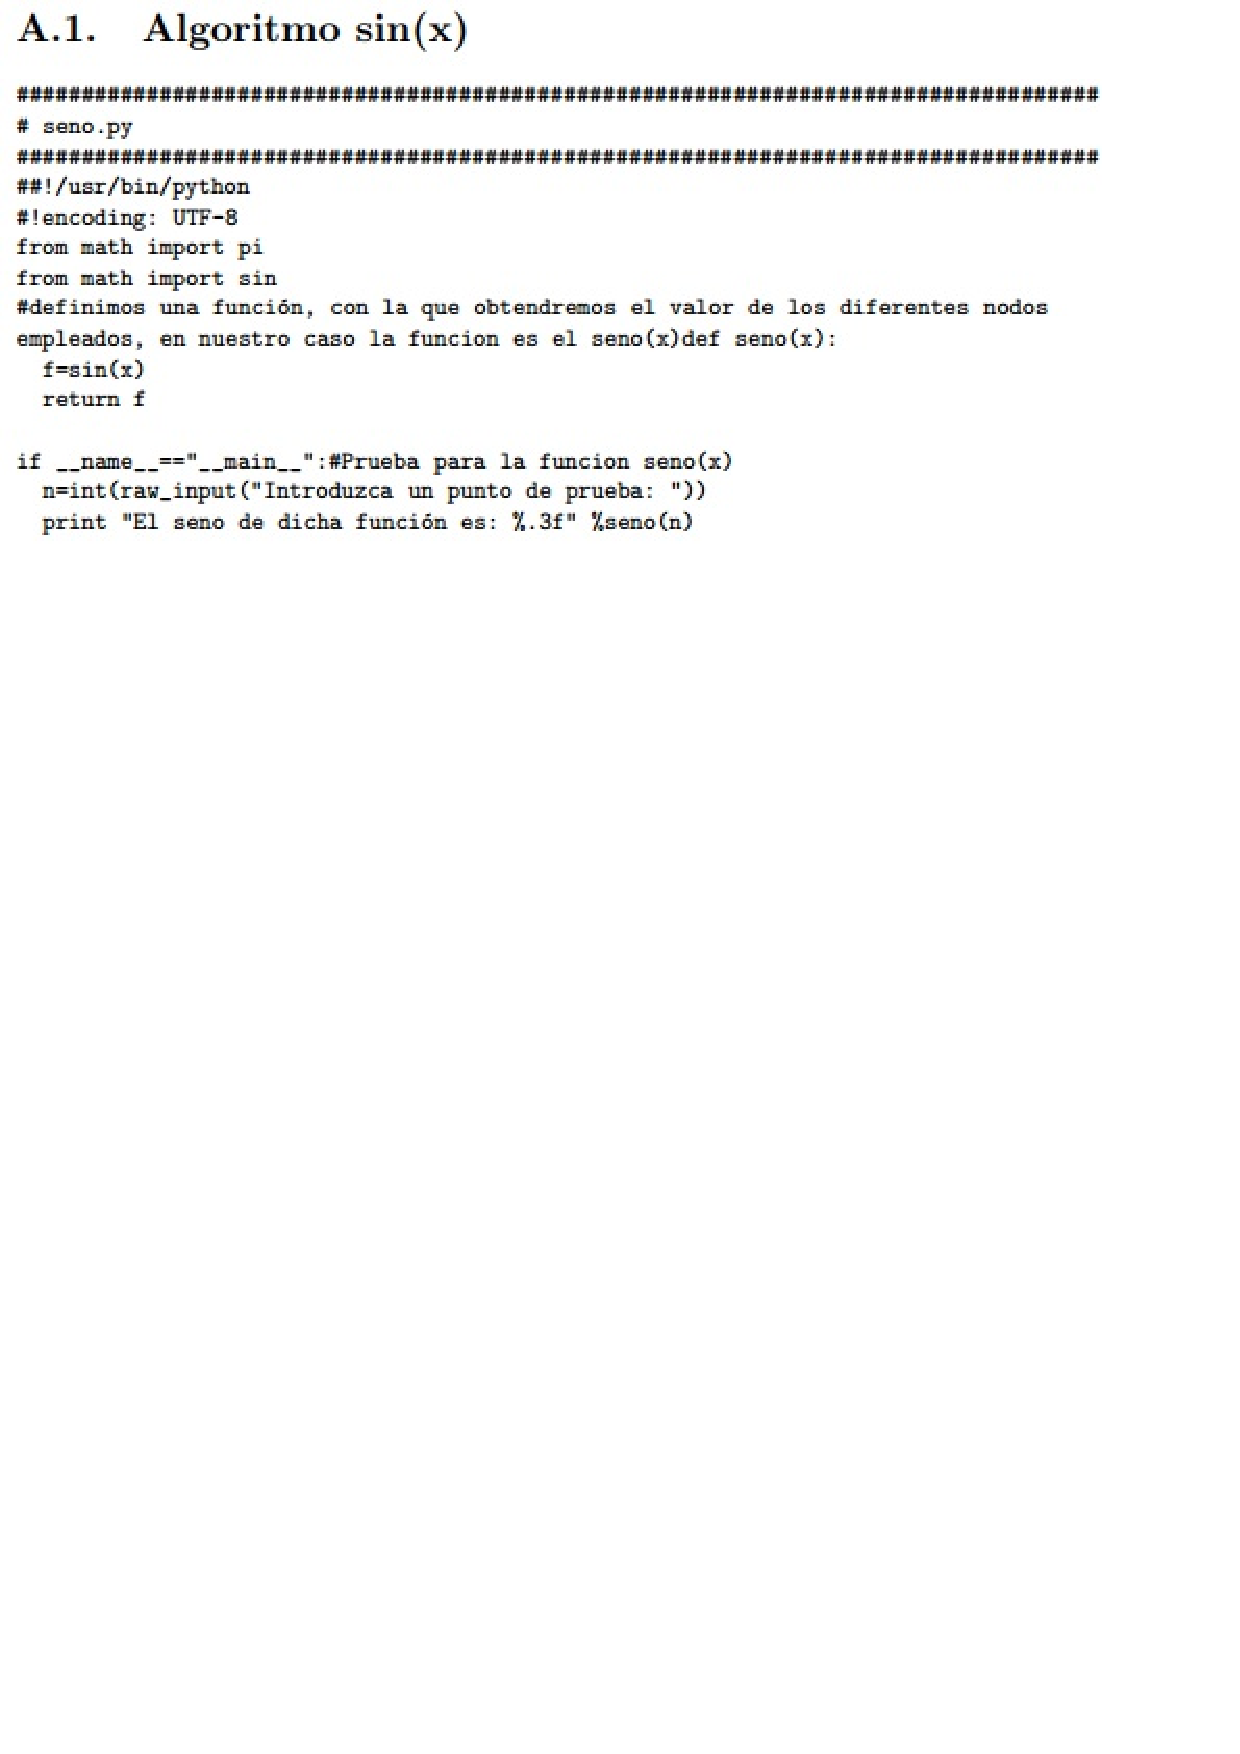
\includegraphics[width=1.0\textwidth]{img/Algoritmo1}
\end{frame}
%++++++++++++++++++++++++++++++++++++++++++++++++++++++++++++++++++++++++++++++
\begin{frame}
  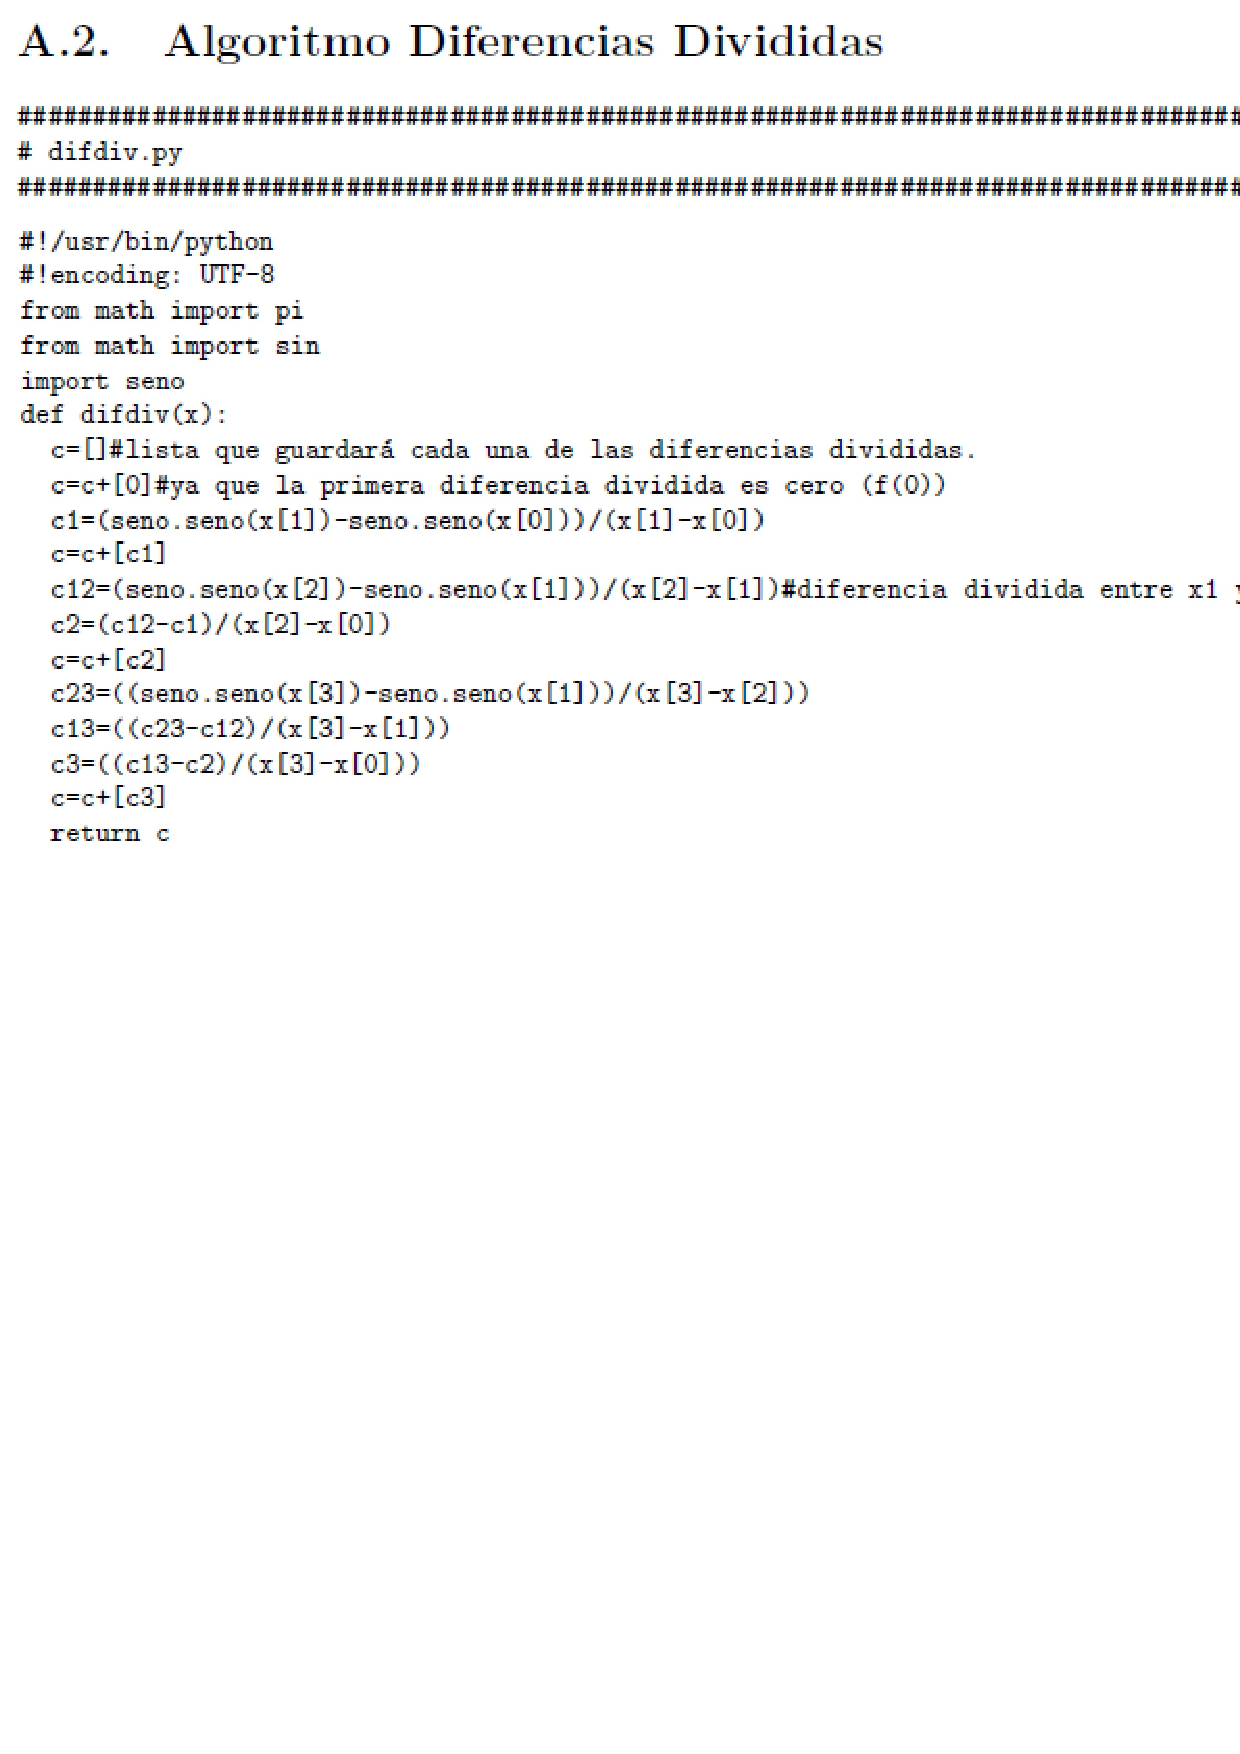
\includegraphics[width=1.0\textwidth]{img/Algoritmo2}
\end{frame}
%++++++++++++++++++++++++++++++++++++++++++++++++++++++++++++++++++++++++++++++  
\begin{frame}
  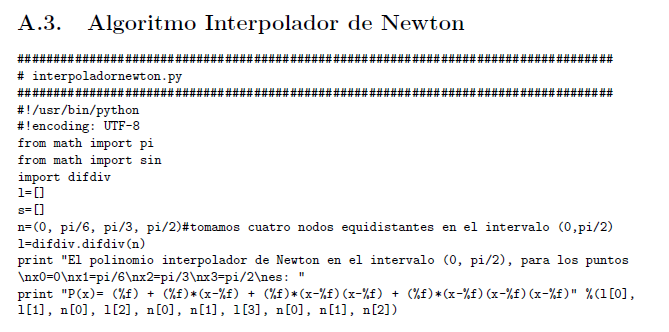
\includegraphics[width=1.0\textwidth]{img/Algoritmo3}
\end{frame}
%++++++++++++++++++++++++++++++++++++++++++++++++++++++++++++++++++++++++++++++
\begin{frame}
  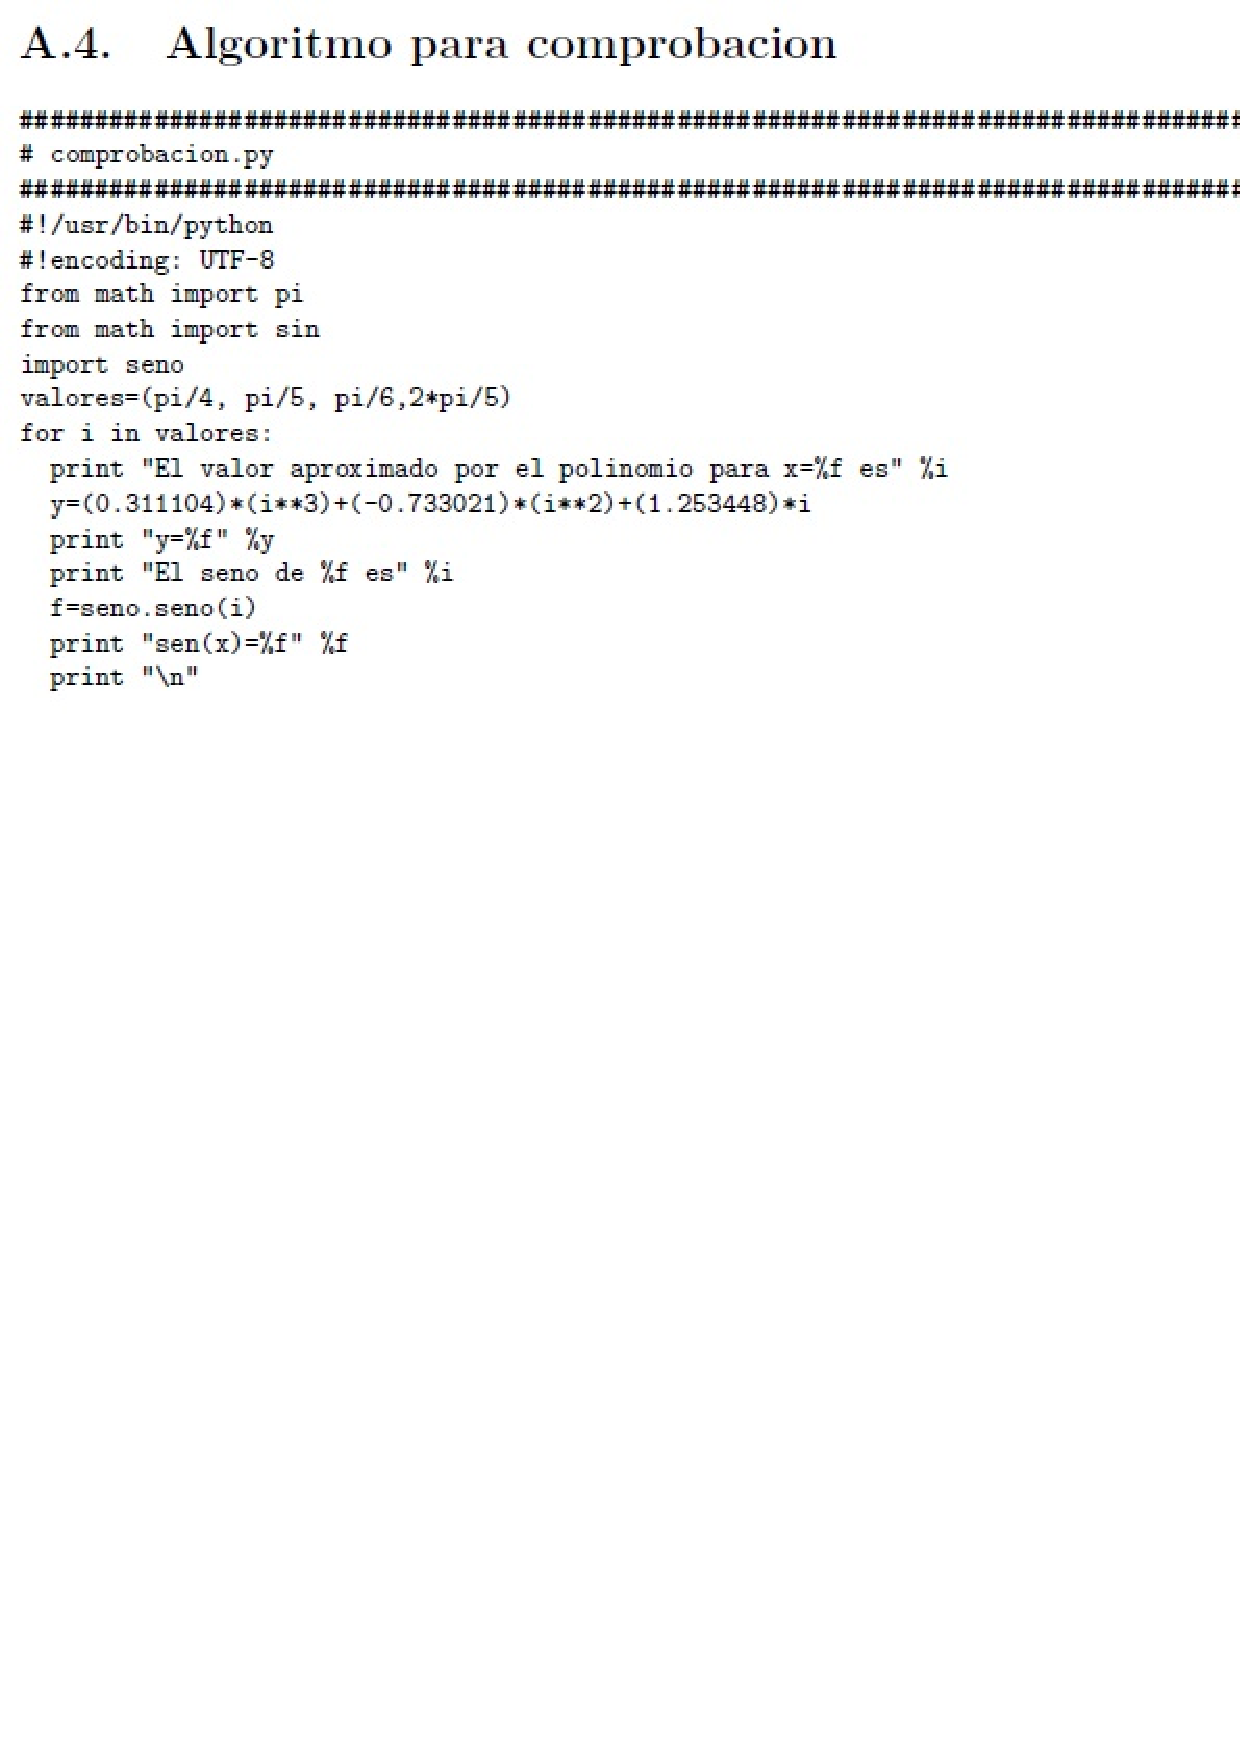
\includegraphics[width=1.0\textwidth]{img/Algoritmo4}
\end{frame}
%++++++++++++++++++++++++++++++++++++++++++++++++++++++++++++++++++++++++++++++
\begin{frame}
A.5. Algoritmo de representación gráfica
  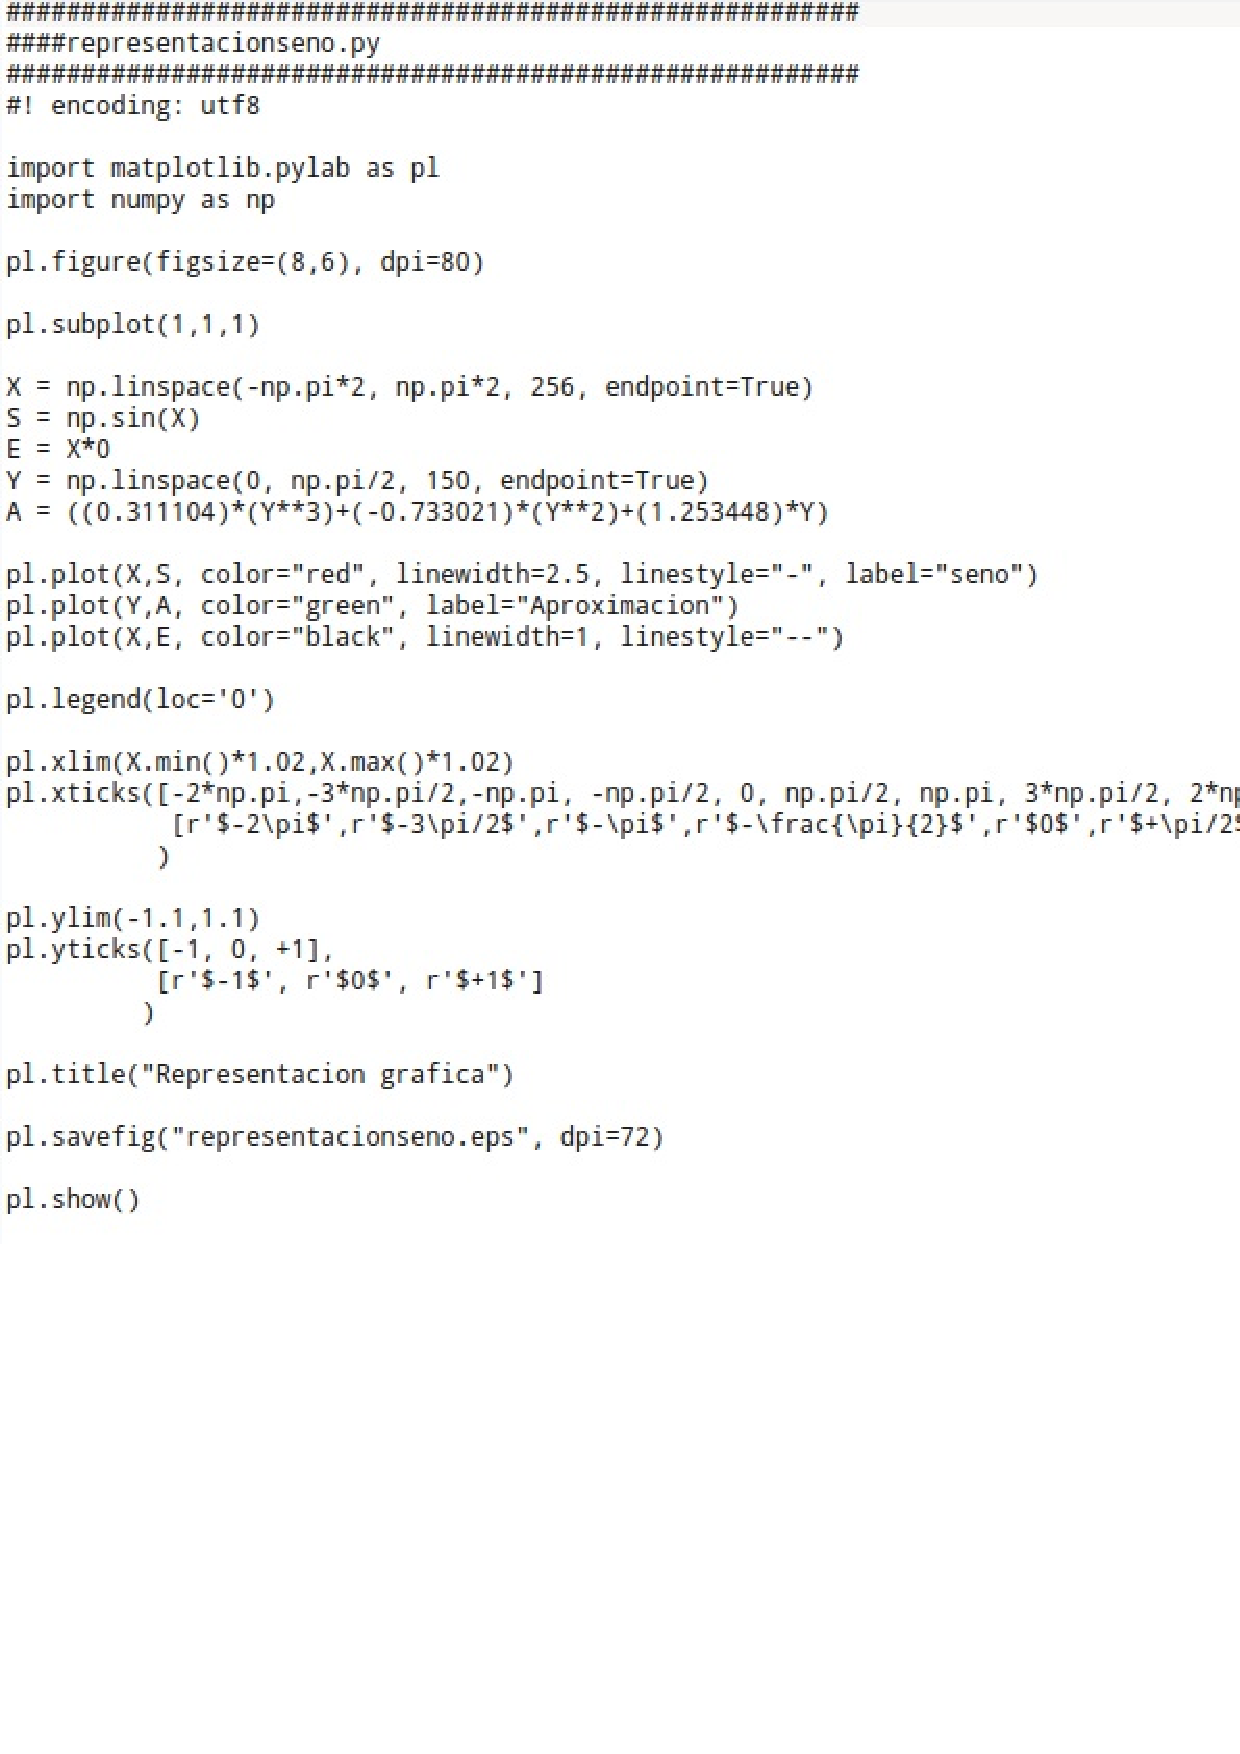
\includegraphics[width=0.75\textwidth]{img/Algoritmo5}
\end{frame}
%++++++++++++++++++++++++++++++++++++++++++++++++++++++++++++++++++++++++++++++
\section{Bibliografía}
%++++++++++++++++++++++++++++++++++++++++++++++++++++++++++++++++++++++++++++++  
\begin{frame}
  \frametitle{Bibliografía}
    \bibliographystyle{plain}

    \bibliography{ej_beamer.bib}
\end{frame}

%++++++++++++++++++++++++++++++++++++++++++++++++++++++++++++++++++++++++++++++  
\end{document}
